\documentclass[a4paper]{article}
 
\usepackage{amsmath}
\usepackage{graphicx}
\usepackage{caption}
\usepackage{subfigure}
\usepackage{epstopdf}
\usepackage[ansinew]{inputenc}
\usepackage{listings}
\usepackage{xcolor}
%\setlength{\oddsidemargin}{0cm}
%\setlength{\evensidemargin}{0cm}
%\setlength{\topmargin}{0cm}

\usepackage[]{algorithm2e}

\usepackage{a4wide}

\title{ Simulating the mouse brain model constructed from Allen Institute for Brain Science data on the Blue Brain 4 supercomputer - Road map }
\author{Till Schumann}
%\date{}

\begin{document}
   \maketitle

\section{Road map}
\begin{itemize}
\item Visualize and validate simulations (because of long waiting time BG/Q, this should be done in parallel to all other tasks)
\item First visualization with Csabas script (mid of August)
\item Literature review (end of August)
\item Optimize implementation by parallelizing (OpenMP) NEST connect function (end of August)
\item Write analysis part of thesis (end of August)
\item Integrate python interface (mid of September)
\item First visualization with ViSNEST (mid of September)
\item Define visualization requirements (end of September)
\item Optimize task scheduling (mid of October)
\item Creating diagrams (mid of October)
\item Write implementation description (mid of October)
\item Improve visualization possibilities (end of thesis)
\item Improve user experience (end of thesis)
\item Finalize thesis (end of thesis)

\end{itemize}


\section{Analysis of existing NEST implementation and scaled-down model of the mouse brain built by BBP Neurorobotics team}
Nice diagrams should be created, based on given HDF5 files.
\section{Definition of work flow and requirements (algorithm complexity) to support loading scaled-down mouse brain model on HPC systems}
Literature review for requirements + memory consumption study, based on NEST paper (one is already given), for different use cases.
\section{Implementation of prototype algorithm to support loading and distributing neuron data and connection in parallel}
\subsection{Current C++ implementation}
\label{sec:currentImpl}
A hybrid implementation of the algorithm distribute parts of the algorithm to $4$ threads.
\emph{"Read chunk.."}, \emph{"Create connection.."} and \emph{"Map target neurons.."} are part of the \emph{"Load data from HDF5"} function.
\emph{"MPI\_Alltoall sorted"} is done in the \emph{"Communicate"} function.
Therefore all objects are placed in memory at once.
Further \emph{synapse table} is placed $4$ times in memory.

\begin{figure}[h]
\centering
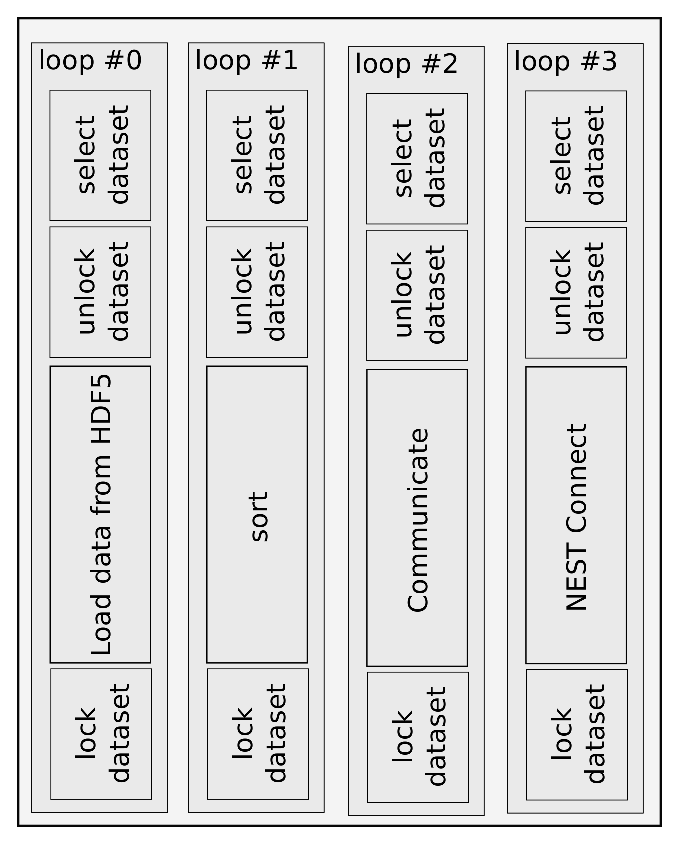
\includegraphics[scale=0.5]{alg_hybrid.eps}
	\caption{Hybrid implementation of algorithm. Each column is executed on another thread. 
	The selection of the datasets works in a round robin fashion.
	Thus the order of applied tasks on each dataset is equal to the sequential algorithm.
	The unblock call can block a thread, if the selected dataset is still in use by the previous thread.}
	\label{Mikesformatcon}
\end{figure}


%\section{Integrate data format for NEST}
%The data format described in \ref{Mikesformatcon} contains connection information based on source and target ids.
%There are no more synapse information as synaptic type and biochemical constants available.
%Synaptic types which depends on the source neuron type can be generated by a random distribution on the fly.
%But the synaptic delay depends on the distance of the source and target neuron, which are stored in a separate hdf5 file.
%Therefore look up is necessary which can be done in memory or disk.
%First one is expensive in regards to time and the second one is expensive in regards to memory consumption.

\section{Optimization strategies of current implementation}
The current implementation V03 allows to load all given data in parallel on 1K nodes.
To get a meaningful neuronal network the given data has to be extended by the proportion of excitatory and inhibitory neurons.
The given dataset does not distinguish between both types.
Therefore all neurons are spitted up using a random function.
Further the synaptic delays of the connections has to be calculated.
They depend on the length of the connection.
Therefore the coordinates of the neurons are used to calculate each distance.
These distances are multiplied by an factor to get the synaptic delays.

A load-balancing strategy is implemented, which sorts all hdf5 files by size before they are distributed to the nodes.

\subsection{Multi threaded call of NEST connect function}
In the current implementation the NEST connection function call takes most of the time.
It could be optimized calling it in parallel. Therefore another sorting operation has to be implemented.
The usage of parallel connect is critical and has to be tested carefully.
From a first look inside the code, it should be doable.
In the current implementation the NEST connect call takes around $25 \mu s$ per connection. 

\begin{figure}[h]
\centering
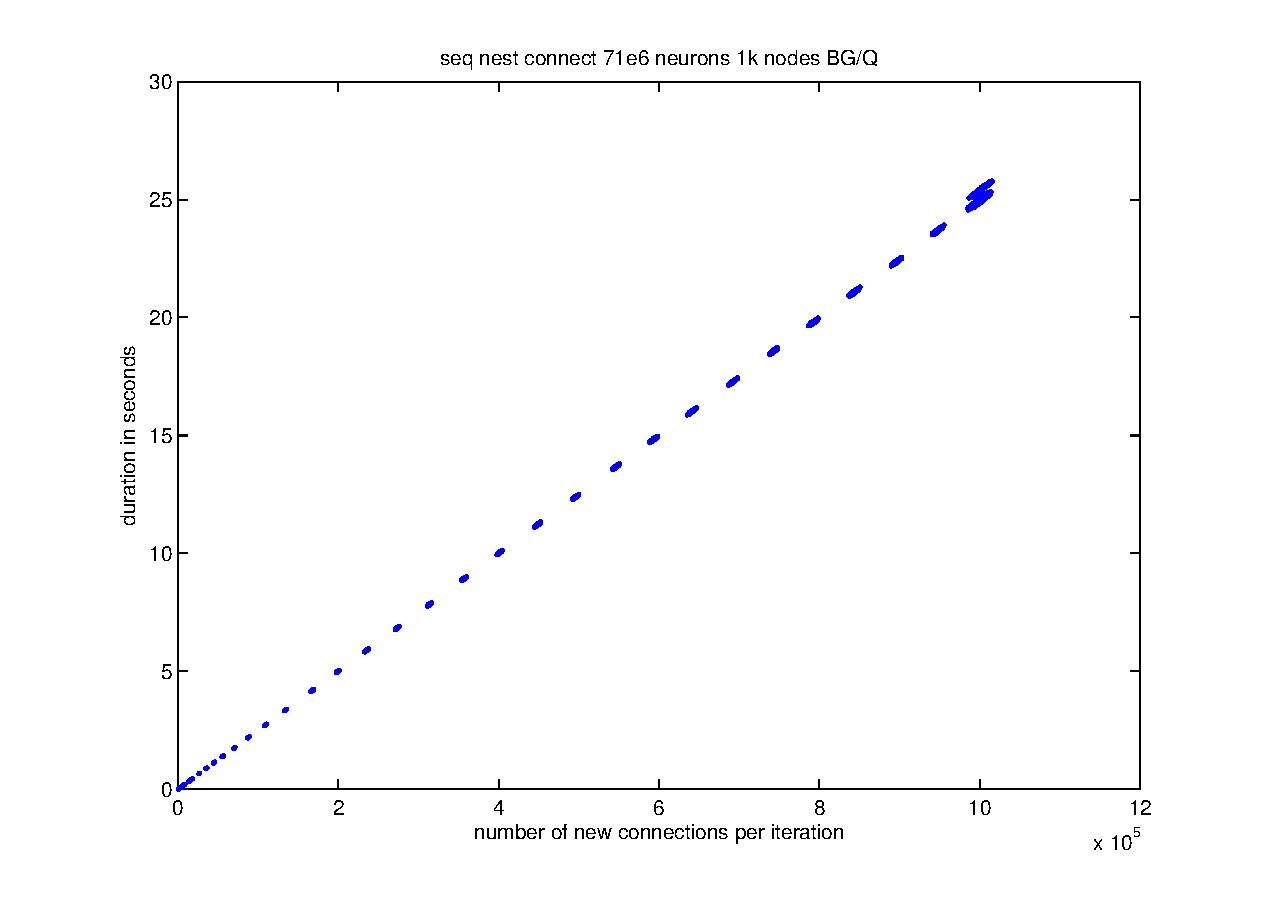
\includegraphics[scale=0.5]{seq_nest_conncet_1k.eps}
	\caption{Duration of NEST connect function measured in build-up process.}
	\label{Mikesformatcon}
\end{figure}


\subsection{Thread scheduling}
The current implementation uses mutexes to realize a task queue which runs in parallel on four different threads using four different datasets. So each thread handles one dataset. After a task is done on a thread the dataset is send in a round robin fashion to the next thread in the queue (see \ref{sec:currentImpl}). The chosen strategy works fine on the BGQ, but violates the OpenMP standard.
Therefore a different queuing strategy should be implemented. An alternative approach is tested in an example program,
but not tested yet with the NEST implementation. 

\newpage
\section{Validate and benchmark prototype implementation on IBM Blue Gene/Q up to 4 racks (4096 nodes)}
Using the implementation inside NEST, it takes around 1 hour to build up the network. Simulating the whole network takes around 1,5 h per 1 second of real time.
\begin{figure}[ht!]
     \begin{center}
        \subfigure[Load hdf5 files]{%
            \label{fig:first}
            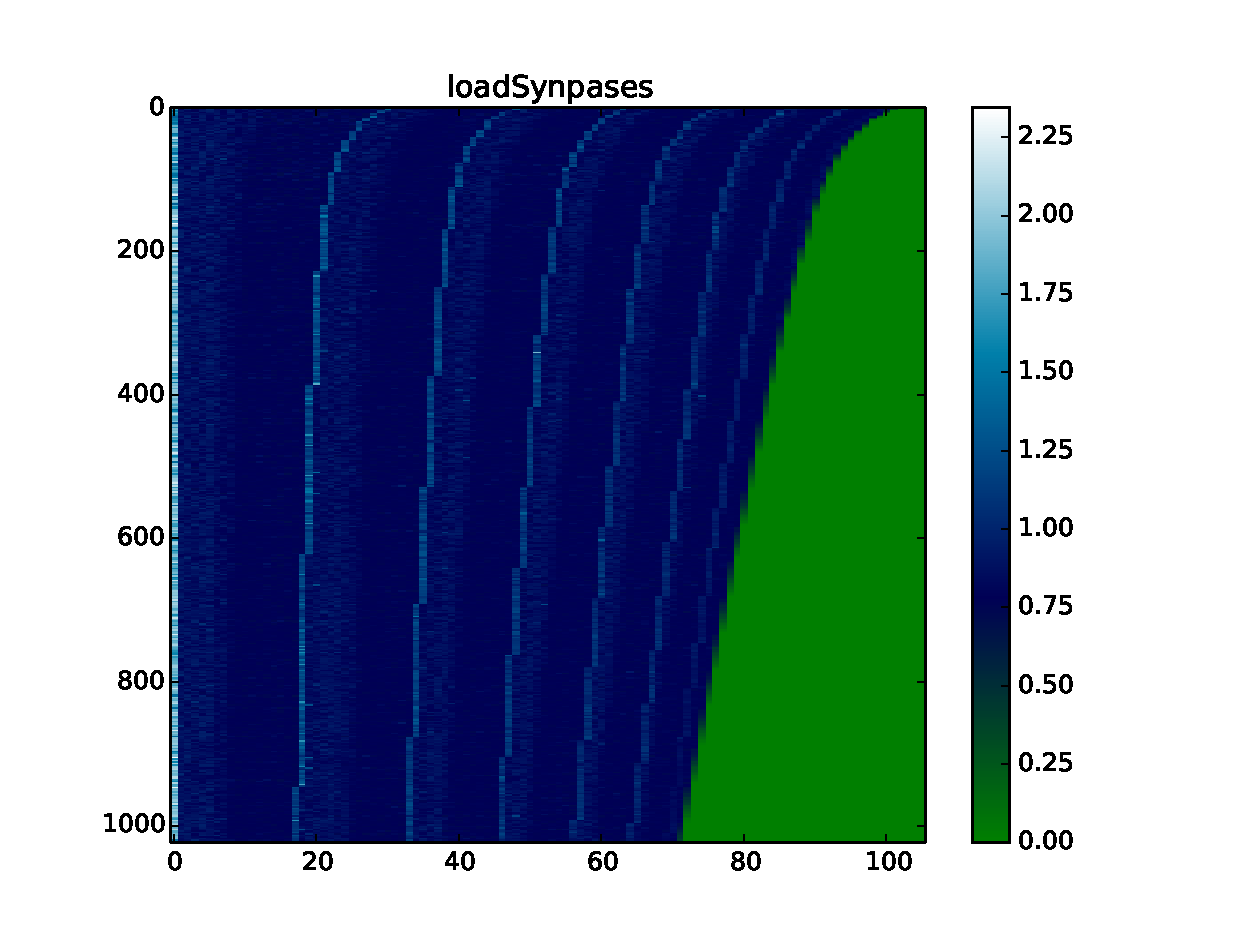
\includegraphics[width=0.4\textwidth]{V03_loadSynapses.eps}
        }
        \subfigure[Sort connection information data by target node]{%
           \label{fig:second}
           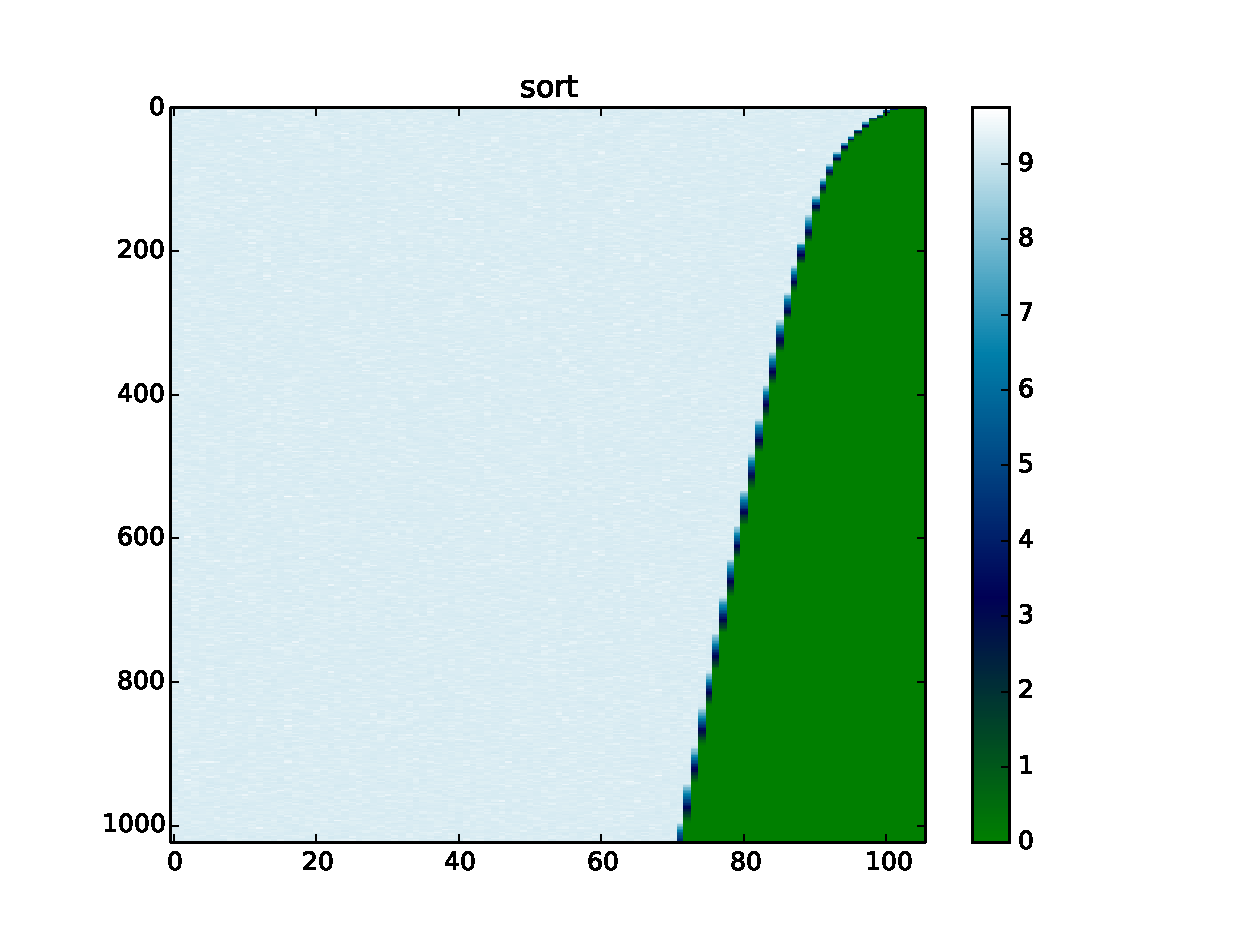
\includegraphics[width=0.4\textwidth]{V03_sort.eps}
        }\\ %  ------- End of the first row ----------------------%
        \subfigure[Send data to all target nodes using AlltoAllv]{%
            \label{fig:third}
            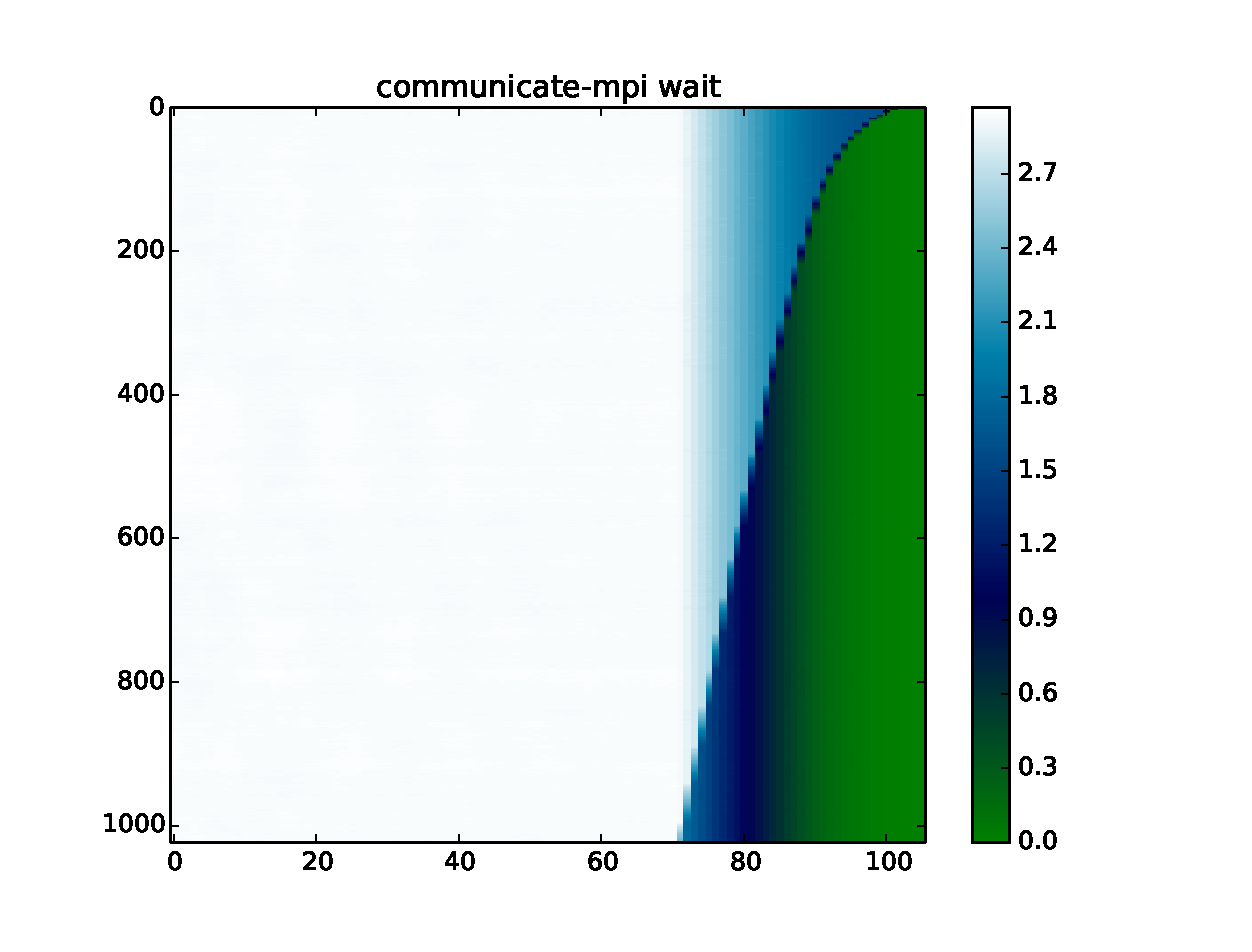
\includegraphics[width=0.4\textwidth]{V03_communicate.eps}
        }
        \subfigure[Connect function which calculated delay and calls NEST connect]{%
            \label{fig:fourth}
            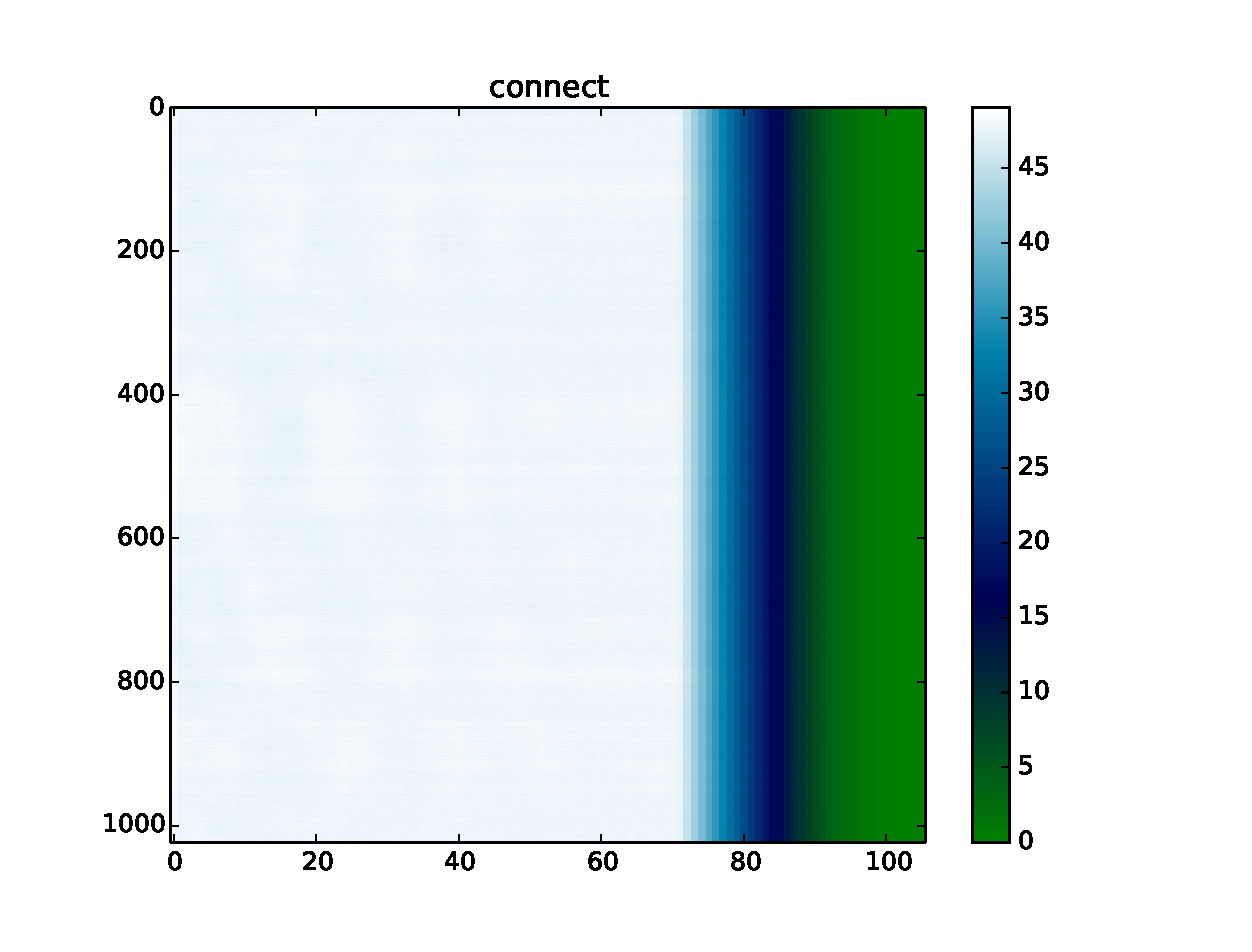
\includegraphics[width=0.4\textwidth]{V03_connect.eps}
        }
    \end{center}
    \caption{%
        The the plots show the the execution time for node per iteration.
        The y-axes corresponds to the node id and the x-axes corresponds to the iteration number.
        The color scale is in seconds.
        In each iteration loadSynapses loads max $1e6$ synapses from hdf5 file.
     }%
   \label{fig:implV03}
\end{figure}
The given plots should be generated for all new implementations for comparison.
They do not include the total runtime.
Thus a different strategy has to be used to compare different types of task scheduling strategies.


\section{Integration of prototype implementation into NEST software}
The current implementation can be accessed via the NEST SLI interface.
The SLI function \emph{HDF5MikeLoad\_s\_s} has to be called with the path of the neurons coordinate file and the path to the folder, which contains the synapse hdf5 files. The SLI function could be extended for more parameters containing a list of parameters in a SLI Dictionary, if necessary.

\section{Improvement of user experience by integration of functionality into NEST python interface}
At first compiling problems with NEST and Python on the BG/Q has to be resolved.
To call the import function from the python interface, a wrapper of the SLI function has to be implemented in the Python interface.
\section{Integration of prototype work flow with visualization pipelines}
For a first try simulation data should be visualized with the visualization script from Csaba.
Therefore a simulation on 1k has to be extended with Spikedetectors, which write spike trains in ASCII file to disk during simulation.
These spike trains can be post processed and used by Csaba.
After that the same data should be used for visualization with ViSNEST.
Depending on the outcome of both visualizations new strategies can be investigated.  

\section{Investigation of metrics and  methods to provide useful insights to scientific users}
To make the simulation in NEST more meaningful, a filter of neuron sets should be implemented in NEST.
At the moment the whole dataset can be loaded inside of NEST.
But it is not possible to distinguish between different types (e.g inhibitory and excitatory neurons) of neurons afterwards.
In a standard use case of random networks neurons of different types are created separately. 
Thus a different treatment in simulations is possible (e.g. only set a input current of neurons from layer L5i; Increase the number of connections between two specific layers). This feature should be provided for the Allen mouse brain model, too.

\end{document}
